\RequirePackage{fix-cm}
\documentclass[11pt]{article}
\usepackage[a4paper,left=18mm,right=18mm,top=15mm,bottom=15mm]{geometry}
\usepackage{amsmath,amssymb,bm,graphicx,booktabs,placeins,float}
\usepackage[font=small,skip=6pt]{caption}
\usepackage[T1]{fontenc}
\usepackage{newtxtext,newtxmath,microtype}
\usepackage[colorlinks=true,linkcolor=blue,urlcolor=blue]{hyperref}
\graphicspath{{../figures/reference/supplemental/}{../figures/generated/supplemental/}}
\renewcommand{\thefigure}{S\arabic{figure}}
\renewcommand{\thetable}{S\arabic{table}}
\renewcommand{\theequation}{S\arabic{equation}}
\renewcommand{\thesection}{\Roman{section}}
\renewcommand{\thesubsection}{\Alph{subsection}}
\widowpenalty=10000
\clubpenalty=10000
\displaywidowpenalty=10000
\setlength{\parindent}{1.2em}
\setlength{\parskip}{0.15em}
\setlength{\textfloatsep}{10pt}
\setlength{\intextsep}{10pt}
\renewcommand{\topfraction}{0.95}
\renewcommand{\bottomfraction}{0.9}
\renewcommand{\textfraction}{0.05}
\renewcommand{\floatpagefraction}{0.8}
\begin{document}
\begin{center}
{\Large\bfseries Supplemental Material for\\[3pt]
Disorder-Restored Strong Connectivity in Degree-Limited Spatial Networks}\par
\vspace{8pt}
Jinhao Zhang$^{1,2}$, Jialin Meng$^{1,2,3,4,*}$, and Tianyu Wang$^{1,2,3,5,*}$\par
\vspace{6pt}
{\small
$^1$School of Integrated Circuits, Shandong University, Shandong Key Laboratory of Next-Generation Semiconductor Technology and Systems, Jinan 250100, China\\
$^2$Suzhou Research Institute of Shandong University, Suzhou 215123, China\\
$^3$National International Innovation Center, Shanghai 201203, China\\
$^4$Key Laboratory of Computational Neuroscience and Brain-Inspired Intelligence (Fudan University), Ministry of Education, Shanghai 200433, P. R. China\\
$^5$State Key Laboratory of Crystal Materials, Shandong University, Jinan 250100, China\\[4pt]
$^*$Correspondence: \href{mailto:jlmeng@sdu.edu.cn}{jlmeng@sdu.edu.cn} and \href{mailto:tywang@sdu.edu.cn}{tywang@sdu.edu.cn}}
\end{center}
This supplement describes the numerical ensembles, parameter controls, spatial-intervention sensitivity, feedback validation, finite-size geometry, and internal-recurrence and boundary-deletion statistics supporting the Letter. Source tables and scripts are available in the \href{https://github.com/neuromorphicscience-sys/janus-disorder-connectivity}{public reproducibility repository}. All quantities use the graph and orientation definitions of the Letter. Literature references are provided in its reference list.
\paragraph*{Numerical conventions and sample inventory.}
Positions are independent uniform points in an open square, with $N=\operatorname{round}(\sigma L^2)$. Source $i$ retains up to $q$ distinct targets within $2R$, ranked by their projection on $\bm e_i=(\sin\theta_i,-\cos\theta_i)$. Gaussian directions have $\theta_i=Wz_i$ modulo $2\pi$, with independent standard-normal $z_i$. Graphs have no self-loops. Continuous projection ties have probability zero; vertex indices resolve numerical ties reproducibly. Unless stated otherwise, $q=7$, $\sigma R^2=24$, and $R$ is the length unit. $S$ is the largest strongly connected component (SCC) size divided by $N$, including singleton components. Points denote individual graph realizations; summary markers or curves are medians, with interquartile ranges (IQRs).

Table~\ref{tab:inventory} lists the overlapping ensembles used here. Source tables provide realization identifiers and random seeds. The 48 spatial-intervention pairs share 16 geometry and normal-disorder streams across three $W$ values, and the same field seeds recur across correlation lengths. Pooled medians and IQRs describe the spread across these dependent graph-condition observations. The scale comparison contains 192 field reassignments, and the deletion ensemble contains 576 graph-width observations.


\begin{table}[H]\centering\small
\caption{Ensembles used in the supplemental figures at $\sigma R^2=24$. Conditions count distinct parameter combinations within each row; the realization-count range is per condition. The deletion row counts graph/width observations (192 distinct graphs at three widths), and direction controls count 24 matched bases at three orientations. Exact parameter grids, sample counts and realization identifiers accompany the source tables.}\label{tab:inventory}
\begin{tabular}{lrrlrrr}
\toprule
Dataset & $q$ & $L/R$ & Control & Conditions & $n$/condition & Total \\
\midrule
Full Gaussian sizes & 7 & 64,128,256,512 & $W$ & 81 & 4--150 & 4634 \\
Spatial intervention & 7 & 128 & $W$ & 3 & 16 & 48 \\
Direction controls & 7 & 128 & $\Delta\theta$ & 3 & 24 & 72 \\
Largest SCC geometry & 7 & 64,128,256,512 & $W$ & 28 & 16--96 & 784 \\
Internal recurrence & 7 & 128 & $W$ & 24 & 8--96 & 1528 \\
Deletion, three widths & 7 & 128 & $W$ & 12 & 24--96 & 576 \\
Wrapped Laplace & 7 & 128 & $b$ & 30 & 16--32 & 800 \\
Bounded uniform & 7 & 128 & $A$ & 18 & 16--32 & 336 \\
von Mises & 7 & 128 & $\kappa$ & 16 & 16--32 & 416 \\
$\ell$ sensitivity & 7 & 128 & $\ell/R$ & 12 & 16 & 192 \\
Clean feedback & 7 & 128 & $W$ & 1 & 24 & 24 \\
Connection-budget scans & 4--12 & 128 & $W$ & 133 & 8--96 & 4188 \\
Gaussian L128 scan & 7 & 128 & $W$ & 24 & 8--96 & 1528 \\
Isotropic rank fields & 7 & 128 & $\alpha$ & 119 & 16--32 & 3040 \\
Anisotropic rank fields & 7 & 128 & $\alpha$ & 73 & 16--32 & 1840 \\
\bottomrule\end{tabular}\end{table}

\FloatBarrier
\section{Robustness of disorder-restored connectivity}
\subsection{Connection-budget dependence}
The Gaussian scans cover $q=4,5,6,7,8,10,12$ at $L/R=128$. Figure~\ref{fig:q}(a) shows budgets $4,5,7,10$, and panel (b) includes all seven at their respective largest sampled disorder values. Restoration occurs across the tested budgets, with budget-dependent windows and sampled endpoints. Panel (b) summarizes the available high-disorder conditions for each budget.


\begin{figure}[H]\centering
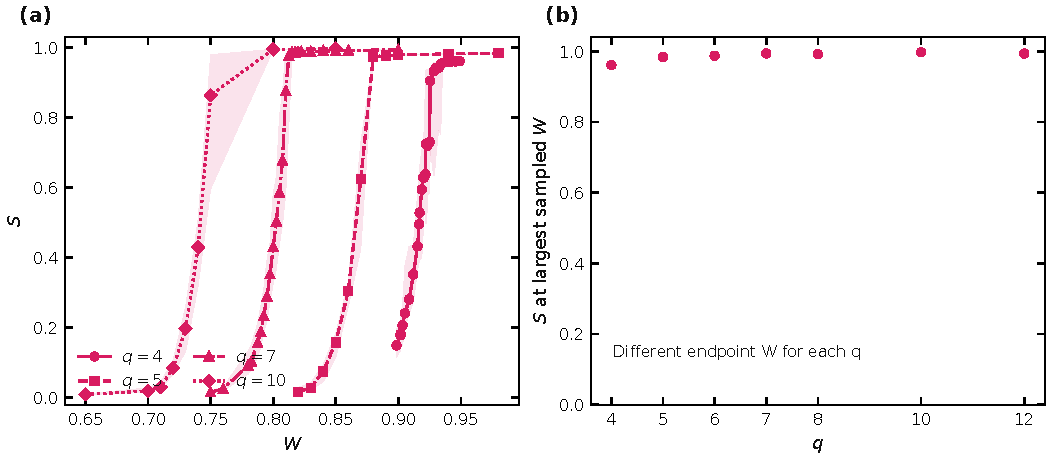
\includegraphics[width=\linewidth]{figS1.pdf}
\caption{Connection-budget robustness for Gaussian orientations at $L/R=128$, $\sigma R^2=24$. (a) $S(W)$ for $q=4,5,7,10$; markers and line styles distinguish budgets. (b) Median $S$ with IQR at each budget\textquotesingle s largest sampled $W$. All curves are medians with IQR bands. Across $q=4,5,6,7,8,10,12$, total graph counts are 784, 240, 352, 1528, 336, 180, 768; counts per sampled $(q,W)$ are 8--96. Endpoint values, $W$ and counts are in the source table.}\label{fig:q}
\end{figure}

\subsection{Disorder families and anisotropy controls}
Independent marks follow wrapped Gaussian, bounded uniform on $[-A,A]$, von Mises, or wrapped Laplace with real-line scale $b$. The von Mises density is proportional to $e^{\kappa\cos\theta}$, with normalization $2\pi I_0(\kappa)$. Figure~\ref{fig:families} uses each distribution's native parameter. The qualitative restoration phenomenon persists across these distinct families over the sampled ranges.

The correlated controls retain a Gaussian orientation multiset at $W=0.82$. Sorted angles are assigned by the ranks of $\sqrt{1-\alpha^2}\,\epsilon_i+\alpha\widetilde h(\bm r_i)$, where $\epsilon_i$ are independent normal variates and the sampled field $\widetilde h$ is centered and normalized over the points. Gaussian smoothing of white noise uses widths $(\ell_x/\sqrt2,\ell_y/\sqrt2)$ on a unit-$R$ grid, followed by bilinear interpolation. Figure~\ref{fig:families}(e),(f) gives actual covariance scales from that kernel. Connectivity decreases with increasing smooth spatial assignment in these scans. They complement the fidelity-constrained intervention of Sec.~II, whose complete diagnostics are shown separately.


\begin{figure}[H]\centering
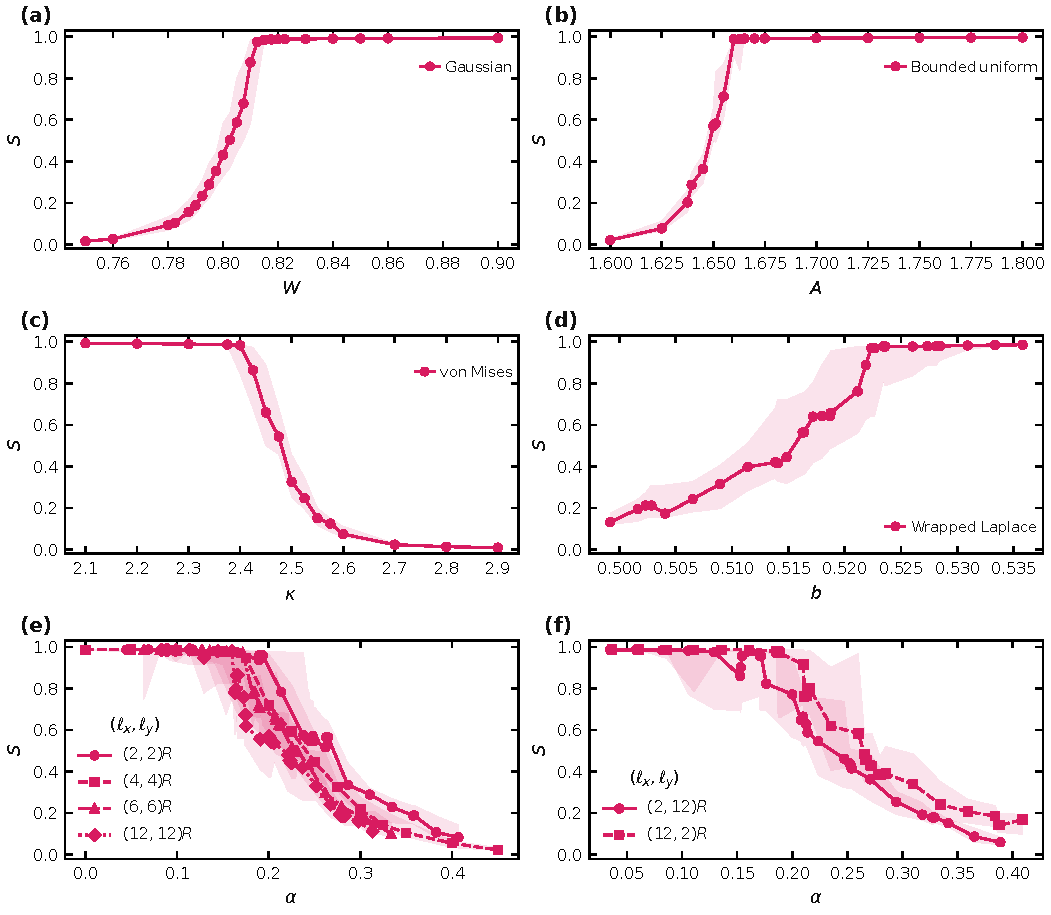
\includegraphics[width=\linewidth]{figS2.pdf}
\caption{Disorder-family and spatial-correlation controls at $q=7$, $L/R=128$, $\sigma R^2=24$. (a)--(d) Native controls $W,A,\kappa,b$ for Gaussian, bounded uniform, von Mises and wrapped Laplace; total counts are 1528,336,416,800. (e),(f) Rank-field mixing $\alpha$ at Gaussian $W=0.82$; labels give actual $(\ell_x,\ell_y)$, with line styles and markers distinguishing scales. Isotropic totals at $(2,2),(4,4),(6,6),(12,12)R$ are 896,384,896,864; anisotropic totals at $(12,2),(2,12)R$ are 928,912. Each sampled condition contains 8--96 graphs. Curves are medians and bands are IQRs.}\label{fig:families}
\end{figure}

\subsection{Finite-size restoration window}
The combined Gaussian cohort contains 4,634 graph realizations at $L/R=64,128,256,512$ and sampled $W$ in $[0.75,0.90]$. Figure~\ref{fig:finite}(a) includes every observation; condition medians, IQRs, variances and bootstrap intervals accompany the source tables. A crossing $W_p(L)$ is the linear interpolation between adjacent sampled medians bracketing $S=p$. Each size has a unique upward bracket for $p=0.1,0.5,0.9$.

The half-height crossings are $0.808,0.802,0.798,0.795$ in increasing size order. Corresponding 10--90\% widths are $0.044,0.029,0.020,0.013$. Table~\ref{tab:bootstrap} reports uncertainty from 4,000 shared-stream bootstrap replicates per size. Exact geometry/orientation seed pairs are resampled jointly across $W$; each replicate recomputes condition medians. Each crossing uses linear interpolation in a unique upward bracket. Width intervals are conditional on both endpoint levels remaining bracketed; the successful fraction is reported. The finite-size window therefore drifts toward smaller $W$ at half height and sharpens across these sizes. These quantities characterize the restoration location and width over the investigated sizes. The larger diagnostic cohort is distinct from the main Fig.~1 display cohort, in which the $L/R=128$ series includes the additional lower-disorder scan.


\begin{figure}[H]\centering
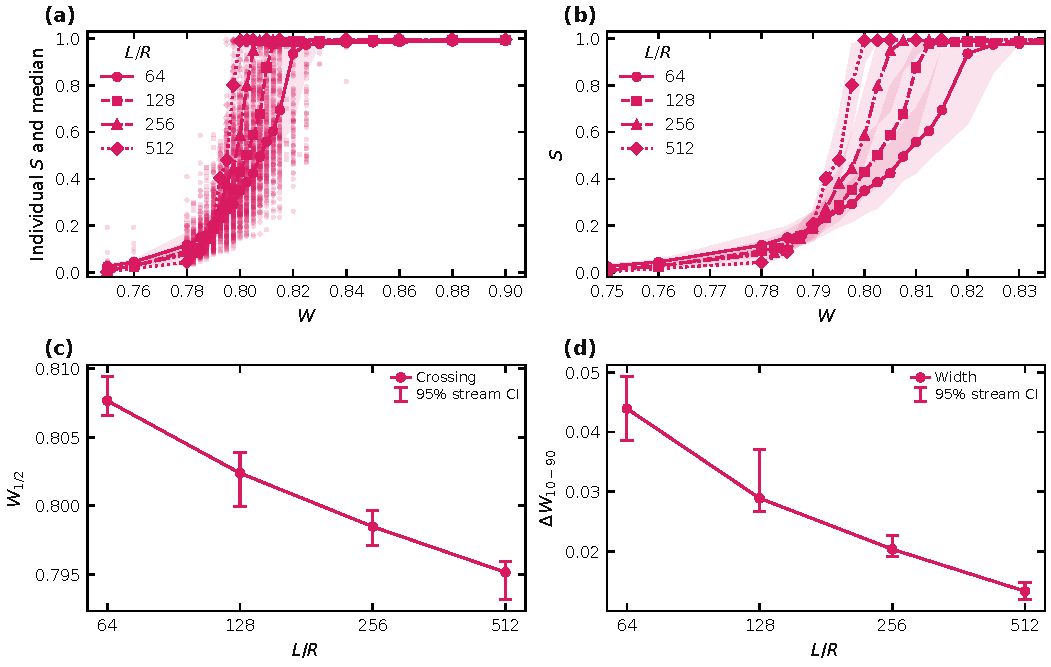
\includegraphics[width=\linewidth]{figS3.pdf}
\caption{Finite-size diagnostics for Gaussian $q=7$, $\sigma R^2=24$. (a) All 4,634 individual $S$ values with condition median/IQR summaries. (b) Median curves and IQR bands, shown over $0.75\leq W\leq0.835$ to resolve restoration. (c) Bracketed $W_{1/2}$. (d) Bracketed 10--90\% width. Total counts for $L/R=64,128,256,512$ are 2040,1584,706,304, respectively; sampled-condition counts range from 4 to 150. Markers and line styles identify sizes in (a),(b). Error bars in (c),(d) are 95\% shared-stream bootstrap intervals from 4,000 draws per size; successful fractions appear in Table~\ref{tab:bootstrap}. Straight segments join sampled or interpolated statistics; complete grids are supplied with the source data.}\label{fig:finite}
\end{figure}

\begin{table}[H]\centering\small
\caption{Descriptive finite-size crossovers with percentile 95\% intervals from shared-stream resampling. Successful fractions refer to bracket-valid replicates. Location and width characterize the finite-size restoration window over the investigated sizes.}\label{tab:bootstrap}
\begin{tabular}{rllll}\toprule
$L/R$ & $W_{1/2}$ [95\% CI] & valid & $\Delta W_{10-90}$ [95\% CI] & valid \\
\midrule
64 & 0.808 [0.807,0.809] & 1.000 & 0.044 [0.039,0.049] & 1.000 \\
128 & 0.802 [0.800,0.804] & 1.000 & 0.029 [0.027,0.037] & 0.936 \\
256 & 0.798 [0.797,0.800] & 1.000 & 0.020 [0.019,0.023] & 1.000 \\
512 & 0.795 [0.793,0.796] & 1.000 & 0.013 [0.012,0.015] & 1.000 \\
\bottomrule\end{tabular}\end{table}

\FloatBarrier
\section{Fixed-multiset spatial intervention}
\subsection{Complete matched-pair fidelity}
For each point cloud, sorted orientations are reassigned by the ranks of an independent Gaussian-smoothed field sampled by bilinear interpolation on a $256\times256$ unit grid. The point crop is shifted by $(64R,64R)$. Positions, the angle multiset, candidate counts and every source outdegree are preserved. Three edge marginals are measured separately for every pair: length, wrapped angle relative to its source direction, and vertical displacement.

Both the Kolmogorov--Smirnov (KS) distance and normalized Wasserstein distance must be at most $0.03$. The Wasserstein normalizers are $2R,\pi,2R$, respectively. The empirical rate is $I_0=-\min_{0\leq t\leq32}\log\sum_b h_b e^{t x_b}$, with normalized frequencies $h_b$ and centers $x_b$ in 2048 bins on $[-2R,2R]$, using $R$ as the numerical length unit. Its relative change $|I_{0,r}-I_{0,o}|/\max(I_{0,o},0.01)$ must be at most $0.03$. At least $25\%$ of original edges must change. The same criteria apply at every correlation length, with marginal fidelity evaluated before surrogate connectivity.

The scale $\ell=4R$ is fixed by the marginal-fidelity criteria before evaluating surrogate connectivity. All 48 main pairs meet the criteria (Fig.~\ref{fig:fidelity} and Table~\ref{tab:fidelity}). Pair indices group the 16 bases at each $W=0.79,0.80,0.81$; these pairwise diagnostics complement the pooled marginal displays of main Fig.~2.


\begin{figure}[H]\centering
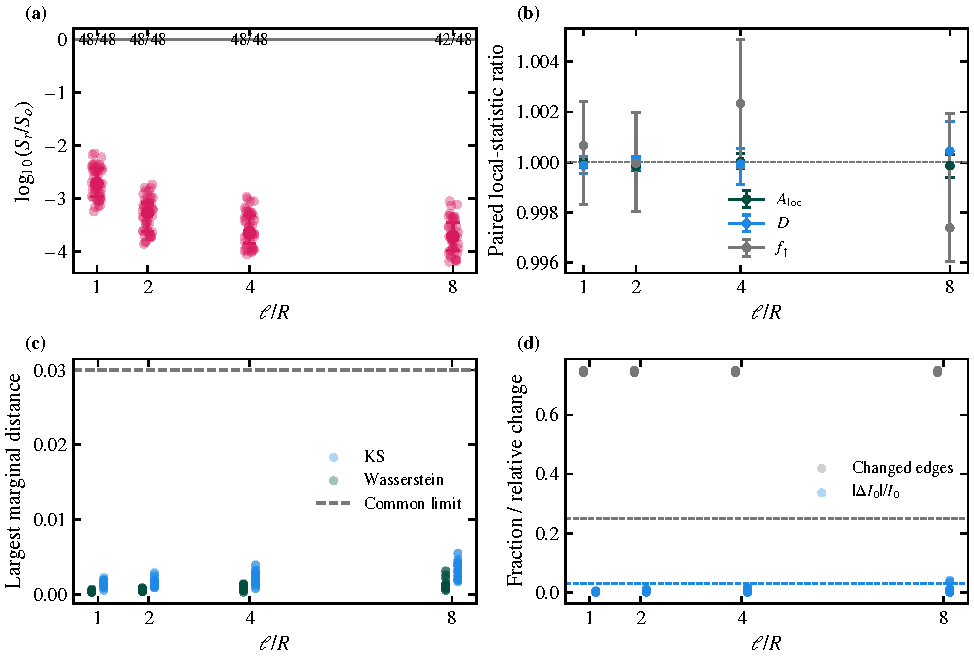
\includegraphics[width=\linewidth]{figS4.pdf}
\caption{Complete fidelity diagnostics for all 48 $\ell=4R$ pairs at $q=7$, $\sigma R^2=24$, $L/R=128$, with 16 pairs at each $W=0.79,0.80,0.81$. (a)--(c) Individual pairwise KS distances (circles) and normalized Wasserstein distances (squares) for edge length, source-relative angle and vertical displacement. (d) Relative empirical-rate change (circles, left axis) and changed-edge fraction (squares, right axis). Amber dashed lines mark the 0.03 upper limits; the dotted line marks the 0.25 changed-edge lower limit. Every pair is displayed and evaluated against the fidelity criteria.}\label{fig:fidelity}
\end{figure}


\begin{table}[H]\centering\small
\caption{Spatial-intervention fidelity at $\ell=4R$ over all 48 pairs. W1 denotes Wasserstein distance after the listed normalization. IQR endpoints and maximum are computed across individual pairs. For changed-edge fraction the lower-limit criterion is relevant; its observed minimum is 0.74290. Machine-readable data also give identical diagnostics for all four correlation lengths.}\label{tab:fidelity}
\begin{tabular}{lllrrrr}
\toprule
Metric & Normalizer & Criterion & Median & IQR & Maximum & Pass \\
\midrule
Length KS & -- & $\leq0.03$ & 0.0011 & [0.0008,0.0015] & 0.0030 & 48/48 \\
Length W1 & $2R$ & $\leq0.03$ & 0.0002 & [0.0001,0.0003] & 0.0011 & 48/48 \\
Relative-angle KS & -- & $\leq0.03$ & 0.0016 & [0.0014,0.0025] & 0.0040 & 48/48 \\
Relative-angle W1 & $\pi$ & $\leq0.03$ & 0.0006 & [0.0003,0.0007] & 0.0013 & 48/48 \\
$\Delta y$ KS & -- & $\leq0.03$ & 0.0013 & [0.0009,0.0017] & 0.0032 & 48/48 \\
$\Delta y$ W1 & $2R$ & $\leq0.03$ & 0.0007 & [0.0006,0.0010] & 0.0014 & 48/48 \\
Relative $I_0$ change & $\max(I_{0,o},0.01)$ & $\leq0.03$ & 0.0048 & [0.0018,0.0116] & 0.0165 & 48/48 \\
Changed-edge fraction & $|E_o|$ & $\geq0.25$ & 0.7467 & [0.7443,0.7491] & 0.7509 & 48/48 \\
\bottomrule\end{tabular}\end{table}

\subsection{Correlation-length sensitivity}
The same 48 base point clouds and orientation multisets are compared at $\ell/R=1,2,4,8$. Each base uses the same white-noise field across lengths, changing only its smoothing width, and contributes one field at each length. All pairs are evaluated with the same marginal-fidelity criteria.

Accepted counts are 48/48, 48/48, 48/48 and 42/48. The six $8R$ rejections fail the unchanged relative-rate limit, with values 0.0349--0.0409; connectivity statistics use the 186 accepted pairs. Fidelity diagnostics for all 192 attempts appear in Fig.~\ref{fig:ell}(c),(d) and the source table. Among accepted pairs, median $\log_{10}(S_r/S_o)$ values are $-2.720,-3.267,-3.648,-3.718$; all 186 accepted reassignments suppress $S$. Connectivity suppression thus persists across the accepted correlation scales while the same marginal-fidelity criteria remain satisfied.


\begin{figure}[H]\centering
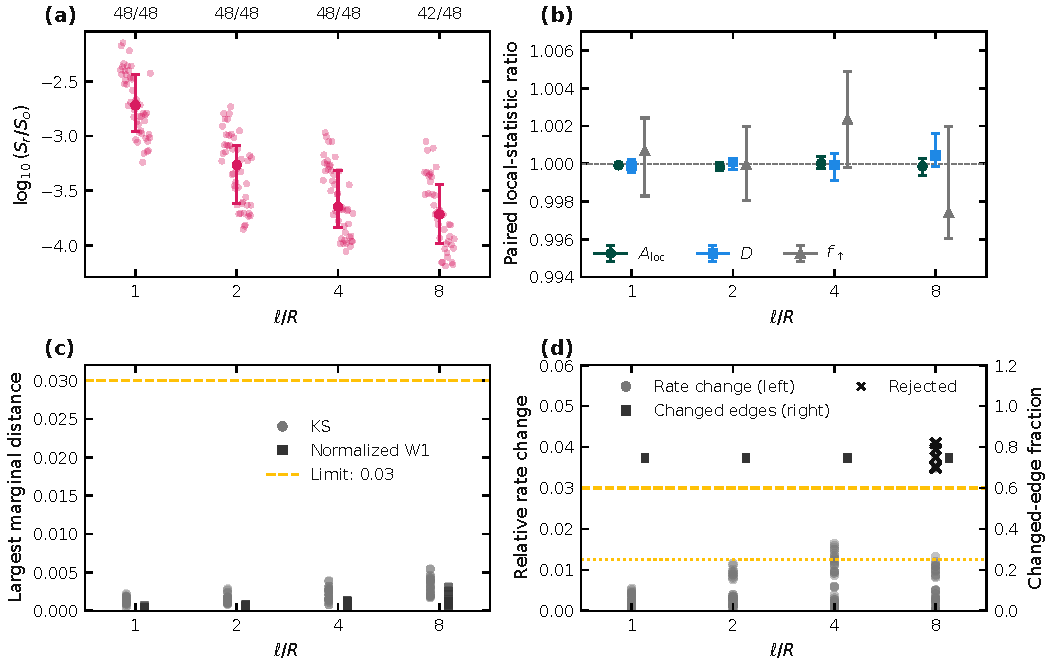
\includegraphics[width=\linewidth]{figS5.pdf}
\caption{Correlation-length sensitivity on 48 matched bases at each $\ell/R=1,2,4,8$, with $q=7$, $\sigma R^2=24$, $L/R=128$ and 16 bases at each $W=0.79,0.80,0.81$. (a) Accepted individual log connectivity ratios, median and IQR; annotations give accepted/attempted counts. (b) Accepted paired local-statistic ratios with median/IQR. (c) Maximum marginal KS and normalized Wasserstein distances for every attempt. (d) Relative-rate change and changed-edge fraction for every attempt; crosses identify six rejected rate values. Dashed upper limits are 0.03, and the dotted changed-edge lower limit is 0.25. Panels (a),(b) summarize accepted pairs; (c),(d) include all 192 attempts. Common seeds across $W$ and $\ell$ make pooled summaries descriptive.}\label{fig:ell}
\end{figure}

\FloatBarrier
\section{Low-order feedback structure and geometry}
\subsection{Feedback-order classifier validation}
The strictly downward graph $D_0$ is acyclic. An upward edge has order one when its target reaches its source through $D_0$. An order-two witness uses one additional upward edge, joined by downward paths. Figure~\ref{fig:classifier} illustrates these two return orders. The sparse implementation tests these witnesses using forward and reverse DAG searches and endpoint buckets, with adjacency arrays and linear-size visit markers; the edge decomposition is $E=D_0\cup F$. Retaining feedback edges of order at most $k$ gives $F_{\leq1}\subseteq F_{\leq2}\subseteq F$ and $G_1\subseteq G_2\subseteq G$.

\paragraph*{Completeness of the search bounds.}
Write $f_i=(u_i,v_i)$ and let $x\leadsto_D z$ include a zero-length path. Strict descent along $D_0$ makes the order-one search exact when restricted to $y\geq y(u_i)$. If no such return exists, an order-two witness is precisely a distinct $f_j=(u_j,v_j)$ satisfying
\begin{equation}
v_i\leadsto_D u_j,\qquad v_j\leadsto_D u_i.
\label{eq:order2witness}
\end{equation}
These paths concatenate with $f_i,f_j$ to close a return with one additional upward edge; conversely every such return has this form. Put $h_j=y(v_j)-y(u_j)$ and $H=\max_{f\in F}h_f$ (with no upward edges there is nothing to classify). Monotonicity and $h_j\leq H$ give
\begin{equation}
y(u_i)-H\leq y(u_j)\leq y(v_i),\qquad
y(u_i)\leq y(v_j)\leq y(v_i)+H.
\label{eq:searchbounds}
\end{equation}
The reverse search from $u_i$ therefore loses no valid $v_j$ when capped at $y(v_i)+H$: every intermediate vertex on its reversed downward path lies below that cap. The implementation rounds both the maximum height gain and the resulting ceiling outward, retaining the bound under floating-point cancellation. Let $C_i$ contain all distinct upward edges whose targets this search reaches, irrespective of their own order. If $C_i$ is empty, no partner exists. Otherwise set $m_i=\min_{j\in C_i}y(u_j)$. Every downward path from $v_i$ to a valid $u_j$ stays at $y\geq y(u_j)\geq m_i$, so the forward search may stop below $m_i$ without loss. Endpoint buckets enumerate all edges incident on each visited endpoint; equality and shared endpoints are retained. Thus the bounds preserve every witness in Eq.~\eqref{eq:order2witness}, including partners that themselves have order one.

The independent bounded-feedback-cost check also retains five toys and 80 induced subgraphs from five parent realizations. The ten uniform $N=64$ subsets contain one downward edge in total. Thirty weak-graph breadth-first $N=64$ neighborhoods contain 84--174 edges (median 102.5), with 31 order-one and 14 order-two labels. Forty feedback-centered $N=128$ subsets contain 81--436 edges (median 152.5), with 76 order-one and seven order-two labels. The latter use eight evenly indexed upward edges per parent, both endpoints and the nearest vertices to their midpoint. All selections depend only on fixed seeds or geometry, independently of the comparison. Every edge agrees, including 107 order-one and 21 order-two positives across the subsets; the five toys also agree. Public scripts and source tables specify the selection rules, vertex indices and edge-wise comparisons. Edges of higher or infinite return order lie outside $F_{\leq2}$.

\paragraph*{Exhaustive checks on complete graphs.}
The command\par\noindent\texttt{python scripts/validate\_full\_graph\_classifier.py}\par\noindent compares every feedback-edge label with two unpruned references: exhaustive return search over states (vertex, upward-edge cost $0$ or $1$), excluding the tested edge, and full $D_0$ reachability followed by enumeration of all upward partners. All $2^{12}=4096$ loopless directed graphs on four strictly ordered vertices agree. A fixed suite of 26 complete model graphs, with $N=96$--1536, $q=7$, $\sigma R^2=24$, and $W=0,0.805,0.9,1.6$, tests 96,768 directed edges, including 3278 order-one and 4395 order-two labels; all agree with both references. Returned witnesses, retained edges and complete SCC partitions of $G_1,G_2$ also agree. Parameters, seeds, graph hashes and edge-wise comparisons are supplied. A negative-coordinate ceiling-cancellation regression is also included. These algorithm checks do not augment the physical ensembles in the figures.

\begin{figure}[H]\centering
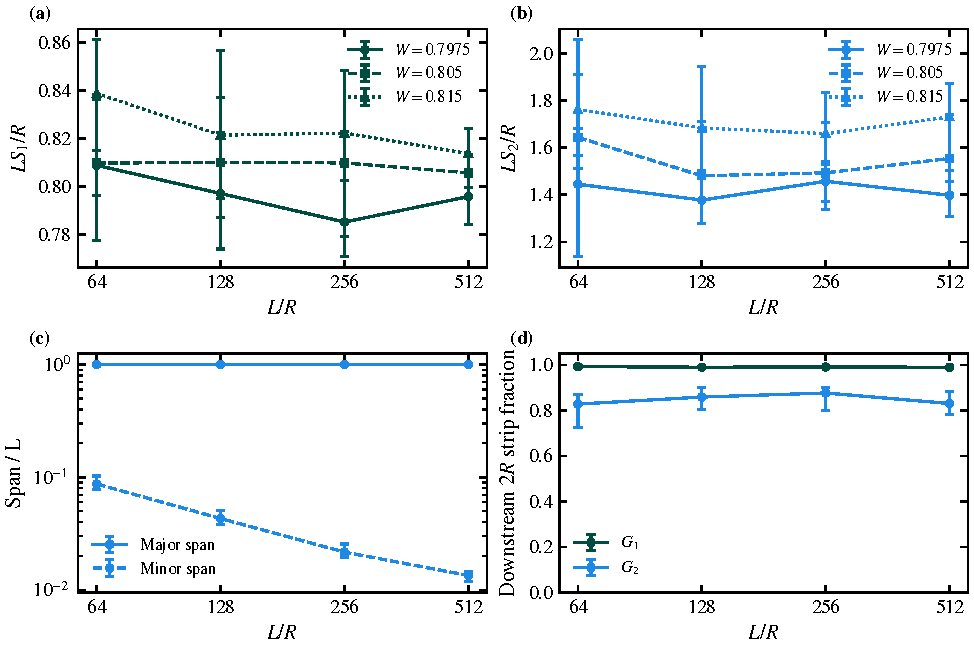
\includegraphics[width=\linewidth]{figS6.pdf}
\caption{Feedback-order witnesses. (a) Two-vertex order-one toy; green is the upward edge, gray is its downward return. (b) Four-vertex order-two toy; blue upward edges connect gray downward paths. Coordinates depict schematic progress along the backbone. The accompanying validation uses five toys and 80 induced subsets from the same five parent realizations: 40 $N=64$ and 40 deterministic feedback-seeded $N=128$ subsets. Total positive feedback labels in the subsets are 107 of order one and 21 of order two; every edge agrees with the independent bounded-cost search.}\label{fig:classifier}
\end{figure}

\subsection{Geometry of the largest low-order components}
The mass and geometry cohort contains 784 graphs at seven $W$ values and four sizes. Figure~\ref{fig:geometry} extends main Fig.~3 at $W=0.805$. The penetration depth $d_{90}$ is the $\lceil0.9|C_{\max}|\rceil$th ordered distance from the downstream wall among vertices of the largest component. For $G_1$, median $d_{90}$ is $1.052$--$1.055R$ while $L$ changes by a factor of eight; the condition IQR endpoints span $0.995$--$1.129R$. For $G_2$, medians range from $2.16$ to $2.51R$, with IQR endpoints $1.98$--$3.26R$. The distributions retain a long tail of deeper components, reaching $57.4R$ in the observed ensemble. The largest low-order components have major span of order $L$ and decreasing relative minor span. These observations concern the largest SCC; the interior contains many other recurrent components.

\subsection{Direction-selection controls}
The 24 matched $L/R=128$, $W=0.805$ bases are compared with orientations shifted by $\pi$ and $\pi/2$. The selected graphs are reconstructed from the shifted directions. Classification uses co-rotating progress coordinates: $y$ originally, $-y$ after reversal, and $-x$ after rotation. The downstream wall is therefore bottom, top or right, respectively. The localization contrast DLOC is largest-component membership in the downstream $2R$ strip minus membership in the opposite strip. Its positive typical values follow the direction under both transformations. All original and rotated $G_2$ contrasts are positive; 22 reversed values are positive and two are zero.


\begin{figure}[H]\centering
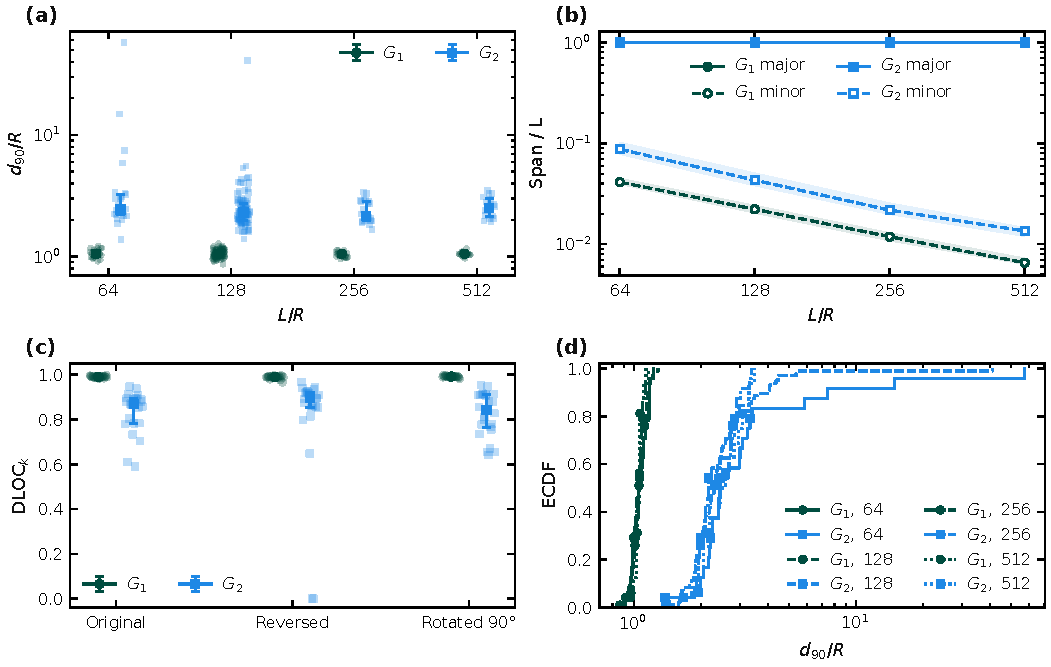
\includegraphics[width=\linewidth]{figS7.pdf}
\caption{Extended geometry and paired direction controls for the largest low-order SCCs, with $q=7$, $\sigma R^2=24$, $W=0.805$. (a) Individual $d_{90}/R$ values and median/IQR at $L/R=64,128,256,512$, with $n=24,96,24,16$. (b) Major/minor spans divided by $L$, median/IQR over the same graphs; solid/filled and dashed/open curves distinguish major/minor spans; circles/squares identify $G_1/G_2$. (c) Individual and median/IQR DLOC for 24 matched bases per orientation, evaluated in co-rotating coordinates. (d) Complete ECDFs of the depths in (a), including long tails; line styles distinguish sizes and circles/squares identify $G_1/G_2$. Geometry is measured for the largest component of each filtered graph.}\label{fig:geometry}
\end{figure}

\FloatBarrier
\section{Internal recurrence and boundary robustness}
\subsection{Full internal-recurrence ensemble}
For the strict interior $I=\{i:4R<x_i<L-4R,\,4R<y_i<L-4R\}$, the graph $G_k[I]$ is induced using labels assigned in the complete graph. Nontrivial SCCs contain at least two vertices. If $M_k^{\rm int}$ is their total vertex count and $C_k^{\rm int}$ their largest component, define
\begin{equation}
 f_{k,\mathrm{rec}}^{\rm int}=M_k^{\rm int}/|I|,\qquad
 \eta_k^{\rm int}=|C_k^{\rm int}|/M_k^{\rm int}.
\end{equation}
All 1,528 realizations have nonzero internal recurrent mass. At the graph level, $S_k^{\rm int}=f_{k,\mathrm{rec}}^{\rm int}\eta_k^{\rm int}$. Each factor is summarized separately, and $S_k^{\rm int}$ is summarized from the per-graph product.

At $W=0.815$, median full-graph $S=0.985$ coexists with internal $G_2$ participation 0.138 and concentration 0.039, with approximately $8.0\times10^3$ nontrivial internal components. At $W=0.90$, participation and concentration medians are 0.946 and 0.996. Substantial internal low-order recurrence can thus remain distributed among many components even when the full graph is macroscopically strongly connected. These are comparisons of ensembles at distinct $W$.


\begin{figure}[H]\centering
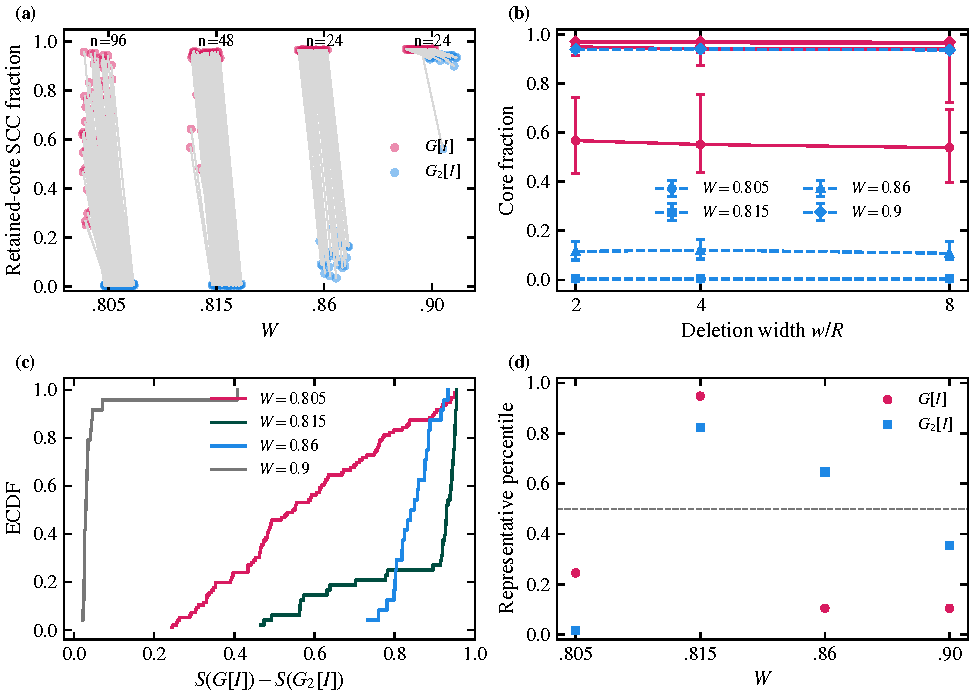
\includegraphics[width=\linewidth]{figS8.pdf}
\caption{Internal recurrence in all 1,528 Gaussian $L/R=128$, $q=7$, $\sigma R^2=24$ realizations at 24 conditions, $0.75\leq W\leq0.90$. (a) Participation $f_{k,\mathrm{rec}}^{\rm int}$. (b) Concentration $\eta_k^{\rm int}$. (c) Nontrivial internal SCC count. (d) Largest nontrivial internal SCC fraction $S_k^{\rm int}$, evaluated as the per-graph product. Curves are condition medians and bands are IQRs; circles/green and squares/blue identify $G_1/G_2$. Actual counts are 8--96 per condition and are listed in the companion source table. Labels are classified in the complete graph before inducing the strict $4R$ interior. All plotted logarithmic quantities are positive.}\label{fig:internal}
\end{figure}

\subsection{Parent-to-internal recurrence retention}
Parent recurrent mass counts core vertices belonging to nontrivial SCCs in the complete $G_k$. Internal recurrent mass additionally requires connecting paths to remain within $I$. Their ratio measures retention under this path restriction. Table~\ref{tab:retention} displays near-restoration and high-disorder conditions; all 24 conditions are supplied in the machine-readable table. A substantial fraction of the parent recurrent population remains internally supported. This population remains distinct from its largest component.


\begin{table}[H]\centering\small
\caption{Parent-to-internal recurrence retention in the strict $4R$ core at $L/R=128$, $q=7$, $\sigma R^2=24$. Entries are median [Q1,Q3] over the stated graph counts. Parent and internal fractions use $|I|$ as their denominator. Retention is the per-graph internal recurrent count divided by its parent recurrent count, summarized after taking the ratio.}\label{tab:retention}
\begin{tabular}{rrrlll}
\toprule
$W$ & $n$ & $k$ & Parent fraction & Internal fraction & Retention \\
\midrule
0.7975 & 96 & 1 & 0.079 [0.079,0.080] & 0.078 [0.077,0.078] & 0.980 [0.979,0.981] \\
0.7975 & 96 & 2 & 0.110 [0.108,0.112] & 0.107 [0.104,0.108] & 0.966 [0.960,0.971] \\
0.805 & 96 & 1 & 0.084 [0.083,0.084] & 0.082 [0.081,0.082] & 0.980 [0.979,0.981] \\
0.805 & 96 & 2 & 0.122 [0.120,0.126] & 0.117 [0.114,0.121] & 0.962 [0.954,0.967] \\
0.815 & 48 & 1 & 0.089 [0.089,0.090] & 0.087 [0.087,0.088] & 0.980 [0.979,0.981] \\
0.815 & 48 & 2 & 0.145 [0.140,0.151] & 0.138 [0.134,0.142] & 0.955 [0.945,0.964] \\
0.86 & 16 & 1 & 0.117 [0.117,0.118] & 0.115 [0.114,0.115] & 0.979 [0.979,0.980] \\
0.86 & 16 & 2 & 0.507 [0.493,0.545] & 0.457 [0.422,0.491] & 0.897 [0.885,0.913] \\
0.9 & 8 & 1 & 0.145 [0.144,0.146] & 0.142 [0.141,0.142] & 0.978 [0.978,0.979] \\
0.9 & 8 & 2 & 0.991 [0.991,0.991] & 0.946 [0.940,0.948] & 0.955 [0.948,0.957] \\
\bottomrule\end{tabular}\end{table}

\subsection{Boundary-deletion ensemble and width dependence}
For width $\Delta$, retain $I_\Delta=\{i:\Delta<x_i<L-\Delta,\,\Delta<y_i<L-\Delta\}$. Feedback labels are assigned in the complete graph, and $G[I_\Delta]$, $G_1[I_\Delta]$, $G_2[I_\Delta]$ are then induced. Deletion retains existing edges between surviving vertices together with their complete-graph labels. Fractions use the retained node count $|I_\Delta|$. The ensemble contains 96,48,24,24 graphs at $W=0.805,0.815,0.86,0.90$, each at $\Delta/R=2,4,8$, giving 576 observations.

At $4R$, median paired differences are 0.548,0.929,0.845,0.029 in increasing $W$ order. Realization spreads and width dependence are retained in Fig.~\ref{fig:deletion} and the source tables. Near restoration, full interior connectivity exceeds the original order-two filtered sector by a large amount; at high disorder the separation is smaller because $G_2$ itself occupies much of the core. At $W=0.805$, the full-core median is 0.5512 and its observed range is 0.2458--0.9578, so the full ensemble has appreciable variation.

The $4R$ panel uses the full 192-graph ensemble. The clean $W=0$ source benchmark uses 24 graphs, with mean upstream-edge count 906.75 and sample standard deviation 12.42, versus fixed-$N$ theory 907.006. It measures clean feedback generation, whereas the deletion ensemble resolves interior recurrent organization under disorder.


\begin{figure}[H]\centering
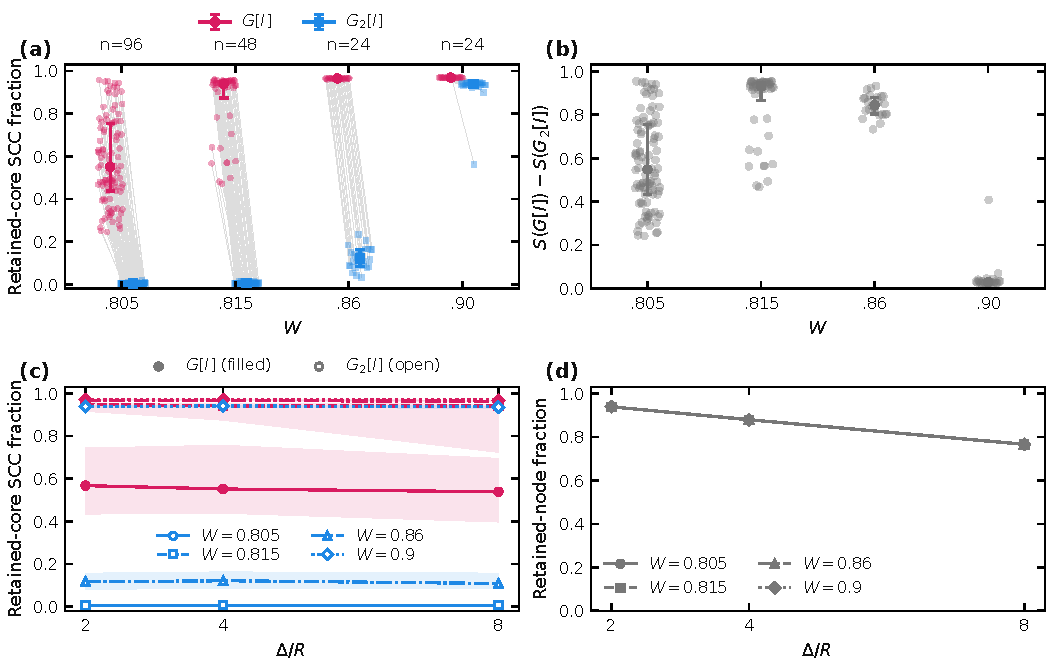
\includegraphics[width=\linewidth]{figS9.pdf}
\caption{Boundary deletion on all 192 eligible Gaussian $L/R=128$, $q=7$, $\sigma R^2=24$ graphs at $W=0.805,0.815,0.86,0.90$. Counts are 96,48,24,24 at every width. (a) Individual paired full and $G_2$ SCC fractions after $4R$ deletion, with median/IQR summaries and faint pair connectors. (b) Corresponding individual paired differences and median/IQR. (c) Width dependence at $\Delta/R=2,4,8$: magenta denotes the full graph, blue $G_2$, and markers/line styles distinguish $W$ and filled/open markers identify $G/G_2$; bands are IQRs. (d) Retained-node fractions, median/IQR, at the same widths and counts. Original complete-graph feedback labels are retained when restricting to the induced subgraphs; all fractions use the retained node count.}\label{fig:deletion}
\end{figure}

\FloatBarrier
\section{Recurrent structure under spatial reassignment}
The same 48 $\ell=4R$ original/reassigned pairs in main Fig.~2 are compared at $W=0.79,0.80,0.81$, with 16 pairs per value. They share 16 geometry/orientation streams across $W$, so pooled medians and IQRs describe dependent graph-condition observations. Labels are assigned separately in each complete original or reassigned graph before restriction to the same strict $4R$ core $I$. Thus $G_k[I]$ retains complete-graph labels, whereas $H_k$ uses orders recomputed after deletion.

Median paired ratios $S_r/S_o,S_{1,r}/S_{1,o},S_{2,r}/S_{2,o}$ are $2.25\times10^{-4}$, $0.0158$, and $0.00947$, with IQRs $[1.45,4.84]\times10^{-4}$, $[0.0143,0.0168]$, and $[0.00814,0.0106]$, respectively. Original median $f_{1,\rm rec}^{\rm int}=0.0792$ (IQR $0.0743$--$0.0838$) and $f_{2,\rm rec}^{\rm int}=0.1096$ ($0.0980$--$0.1211$). Both become exactly zero in every reassigned core, and so does $S_k^{\rm int}$. Original median concentrations are $0.00117$ and $0.0220$; reassigned $\eta_k^{\rm int}$ is undefined because the recurrent mass is zero. Figure~\ref{fig:bridge}(c) shows the original concentrations and marks the reassigned populations as undefined; paired concentration ratios require nonzero recurrent mass. Whole-graph $S_k$ includes singletons, whereas $S_k^{\rm int}$ counts a nontrivial recurrent component and can be zero.

Spatial reassignment removes the measured low-order interior recurrence itself. In the natural-$W$ scan, finite recurrent populations develop participation and concentration on distinct disorder scales. The two comparisons probe complementary aspects of recurrent organization: survival under spatial reassignment and concentration within the natural-disorder ensemble.



\begin{figure}[H]\centering
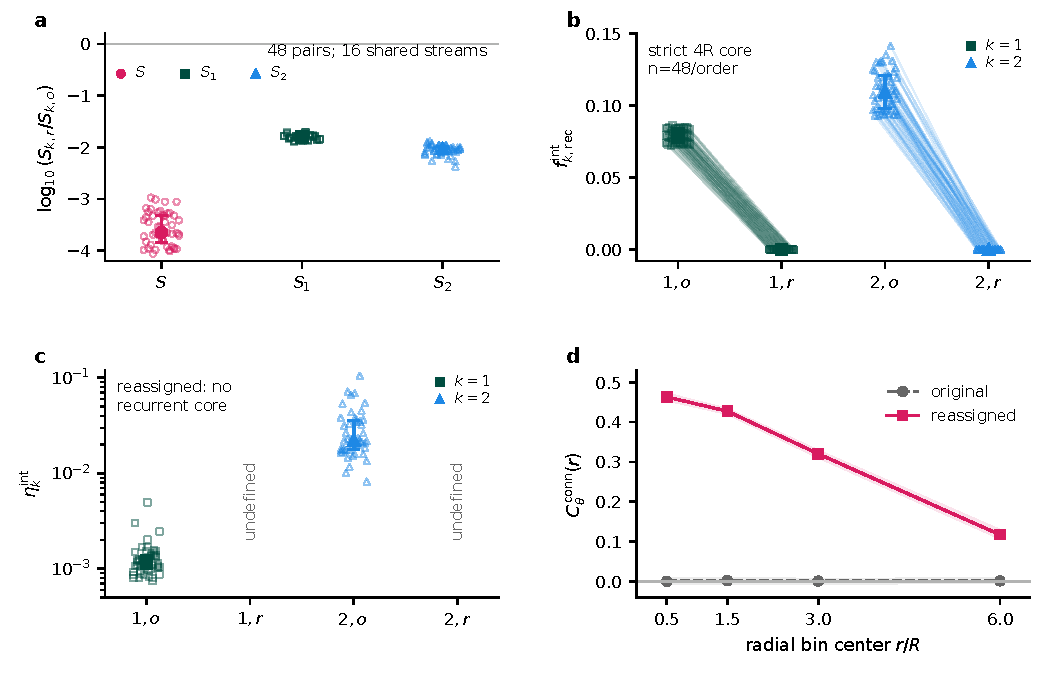
\includegraphics[width=\linewidth]{figS10.pdf}
\caption{Recurrent response to spatial reassignment on all 48 pairs, 16 at each $W=0.79,0.80,0.81$, with $q=7$, $\sigma R^2=24$, $L/R=128$ and $\ell=4R$. (a) Paired log ratios for full and filtered largest-SCC fractions. (b) Paired strict-core recurrent participation for orders one and two; $o,r$ denote original and reassigned. (c) Original concentrations; reassigned concentrations are explicitly undefined because every core has zero recurrent mass. Faint points/connectors are individual pairs; larger markers and bars are medians/IQRs. (d) Connected orientation correlation, median/IQR across the same pairs, using 512 prespecified source anchors per geometry and all targets in four radial bins. Original/reassigned states are distinguished by marker and line style. Connected correlation subtracts the measured polarization baseline. Shared streams make pooled spreads descriptive.}\label{fig:bridge}
\end{figure}

\paragraph*{Orientation-correlation baseline.}
For $P^2=|N^{-1}\sum_i e^{i\theta_i}|^2$, we report $C_\theta^{\rm conn}(r)=\langle\cos(\theta_i-\theta_j)\rangle_r-P^2$. The exact permutation expectation for distinct vertices of this same multiset is $(NP^2-1)/(N-1)$; its excess is also supplied. The permutation baseline is evaluated analytically. Source anchors are selected once with seed 2026100801 and reused for both states and all $W$. The radial bins are $(0,R],(R,2R],(2R,4R],(4R,8R]$. Original median connected values are $0.0006,0.0024,0.0013,0.0017$; reassigned values are $0.463,0.427,0.320,0.118$. These estimates average pair correlations over targets surrounding the fixed source anchors.

\paragraph*{Indegree and reciprocity.}
Mean indegree equals mean outdegree by edge conservation and is seven in these saturated-outdegree realizations. Median indegree variance rises from $10.47$ to $23.71$ (IQRs $10.43$--$10.51$ and $23.27$--$24.48$), and the zero-indegree fraction from $0.00497$ to $0.0221$ ($0.00485$--$0.00512$ and $0.0205$--$0.0225$). The reciprocal-edge fraction, defined as the fraction of directed edges with a reverse edge, decreases from $0.0148$ to $0.000286$ ($0.0140$--$0.0157$ and $0.000266$--$0.000332$). The largest weakly connected fraction remains one in all graphs. Individual histograms and paired differences are supplied. Spatial reassignment thus changes several joint structural properties while preserving positions and the one-point orientation population.



\FloatBarrier
\end{document}
